\documentclass[12pt]{article}

\usepackage{sbc-template}
\usepackage{graphicx,url}
\usepackage[utf8]{inputenc}
\usepackage[T1]{fontenc}
\usepackage[brazil]{babel}
\usepackage{amsmath}
\usepackage{booktabs}
\usepackage{hyperref}

\sloppy

\title{Mineração de Métricas DORA em Repositórios Open-Source:\\o quanto podemos confiar nas aproximações?}

\author{João Vitor Pedersoli Rajao\inst{1}, Pedro Moreira Ramos\inst{1}, Otávio Salomão Ferreira\inst{1}}

\address{Curso de Engenharia de Software -- Pontifícia Universidade Católica de Minas Gerais (PUC Minas)\\
  Belo Horizonte -- MG -- Brasil
  \email{joaorajao5@gmail.com, pedromoreiraramos1998@gmail.com, otavio.ferreira.mds@gmail.com}
}

\begin{document}

\maketitle

\begin{abstract}
We mined the four DORA metrics for 300 of the most popular open-source repositories that use GitHub Actions, over a fixed 12-month window, with a reproducible pipeline (cache, resumption and rate-limit handling). Releases approximate deploys and CI runs approximate failures. The median repository publishes 0.54 releases per week, has a lead time of about 10 days, a CI failure rate of 4.8\% and recovers from a failed run in 2.6 hours. A corrective-release heuristic reached F1 = 0.82 against a three-rater gold sample, but inter-rater agreement on what is a corrective release was only slight ($\kappa = 0.09$). Changing the operational definitions moves 20--39\% of the repositories to another DORA category, so conclusions that depend on the failure definition are fragile.
\end{abstract}

\begin{resumo}
Mineramos as quatro métricas DORA em 300 dos repositórios open-source mais populares que usam GitHub Actions, numa janela fixa de 12 meses, com um pipeline reprodutível (cache, retomada e tratamento de \textit{rate limit}). Releases aproximam deploys e execuções de CI aproximam falhas. O repositório mediano publica 0,54 release por semana, tem lead time de cerca de 10 dias, taxa de falha de CI de 4,8\% e se recupera de uma execução com falha em 2,6 horas. A heurística de release corretiva alcançou F1 de 0,82 contra uma amostra-ouro rotulada por três avaliadores, mas a concordância entre eles sobre o que é uma release corretiva foi apenas leve ($\kappa = 0{,}09$). Trocar as definições operacionais move de 20\% a 39\% dos repositórios de categoria DORA; as conclusões que dependem da definição de falha são frágeis.
\end{resumo}

\section{Introdução}

As métricas DORA (\textit{DevOps Research and Assessment}), popularizadas por \textit{Accelerate} \cite{forsgren2018accelerate}, medem o desempenho de entrega em duas dimensões: velocidade (\textit{deployment frequency} e \textit{lead time for changes}) e estabilidade (\textit{change failure rate} e tempo de recuperação). Em 2023 o tempo de recuperação passou a se chamar \textit{failed deployment recovery time}, e em 2024 o DORA acrescentou a \textit{deployment rework rate} \cite{dora2024history}.

O GitHub não registra deploys nem falhas em produção. Em projetos open-source, as métricas precisam ser inferidas a partir de releases, execuções de CI e commits, ou seja, de \textit{proxies}. Uma biblioteca que publica uma release por mês não está ``deployando'' nada; quem coloca em produção são seus usuários. Por isso, além de calcular as métricas, este trabalho valida a heurística de falha contra o julgamento humano (amostra-ouro) e mede o quanto a classificação DORA muda quando a definição operacional muda.

As hipóteses informais abaixo foram registradas antes da coleta (Sprint 1):
\textbf{H01} (RQ01, frequência): a maioria dos repositórios fica em \textit{Medium} ou \textit{High}, raramente \textit{Elite}, porque o desenvolvimento open-source é assíncrono e voluntário.
\textbf{H02} (RQ02, lead time): mediana entre 1 e 30 dias, com a variante por release (a) bem maior que a por commit (b), pois um único commit antigo ``esquecido'' faz a variante (a) explodir.
\textbf{H03} (RQ03, falha): CFR (a), de CI, moderado a alto ($\ge 30\%$); CFR (b), de entrega, baixo ($\le 15\%$).
\textbf{H04} (RQ04, recuperação): de horas a poucos dias, sem plantão 24/7.
\textbf{H05} (RQ05): sem correlação positiva forte entre frequência e falha ($\rho \le 0$), como afirma o DORA.
\textbf{H06} (RQ06): mais contribuidores, mais estrelas e aplicações/CLIs entregam com mais frequência e menor lead time.
\textbf{H07} (RQ07): a classificação é sensível à definição, com concordância (kappa de Cohen ponderado) fraca a moderada.

\section{Metodologia}

\subsection{Fonte de dados, janela e pipeline}

A coleta usa as APIs REST e GraphQL do GitHub com um cliente próprio, sem bibliotecas prontas de acesso à API. A janela de observação vai de 01/10/2025 a 30/09/2026 (365 dias, 52,1 semanas). O pipeline roda com um único comando (\texttt{python -m labs.lab03\_dora}), lê o token de uma variável de ambiente, salva cada resposta da API em disco e retoma de onde parou; espera a renovação da cota quando ela acaba e repete erros temporários com \textit{backoff} exponencial (1, 2, 4, 8 e 16 s). A coleta completa fez mais de 34 mil requisições e processou 22.130 releases, 4 milhões de commits comparados e 2,97 milhões de workflow runs. Os testes das funções de métricas rodam no GitHub Actions do grupo, com cobertura mínima de 80\% (100\% no módulo de métricas).

\subsection{Seleção da amostra}

A busca \texttt{stars:>1000} é fatiada por faixas de estrelas, das maiores para as menores, e cada faixa com mais de 1.000 resultados é dividida ao meio. Os candidatos são examinados nessa ordem até 300 passarem pelos critérios da Tabela~\ref{tab:funil}. Os 713 candidatos examinados são, portanto, os repositórios com mais estrelas do GitHub (de 40.865 a 552.497). As linguagens mais frequentes na amostra são TypeScript (80), Python (71), Go (32), Rust (31) e JavaScript (29).

\begin{table}[ht]
\centering
\caption{Funil de seleção.}\label{tab:funil}
\small
\begin{tabular}{lrr}
\toprule
Etapa & Restantes & Descartados \\
\midrule
Candidatos examinados & 713 & -- \\
Usam GitHub Actions (\texttt{/actions/workflows}) & 643 & 70 \\
$\ge 5$ releases publicadas na janela (\texttt{draft = false}, sem pré-release) & 346 & 297 \\
$\ge 50$ workflow runs válidos (\texttt{push} no \textit{default branch}) & 300 & 46 \\
\textbf{Amostra final} & \textbf{300} & \\
\bottomrule
\end{tabular}
\end{table}

\subsection{Definições operacionais}

\textbf{Deploy:} release publicada (\texttt{draft = false}, \texttt{prerelease = false}). \textbf{Deployment frequency:} releases na janela / 52,1 semanas.
\textbf{Lead time:} para cada release R, os commits incluídos vêm de \texttt{compare/\{anterior\}...\{R\}}, paginado até o fim; a anterior pode estar fora da janela, e a primeira release da história é ignorada. A data de um commit é \texttt{commit.author.date}. Variante (a): $R - $ commit mais antigo, mediana entre as releases do repositório. Variante (b): $R - $ cada commit, mediana de todos os commits do repositório.
\textbf{CFR (a):} falhas / (falhas + sucessos) dos runs \texttt{push} no \textit{default branch}; \texttt{failure}, \texttt{timed\_out} e \texttt{startup\_failure} são falhas, \texttt{cancelled}, \texttt{skipped} e as demais conclusões são ignoradas. Os runs são coletados mês a mês; meses e dias que atingem o teto de 1.000 resultados da API são subdivididos até a coleta ficar completa.
\textbf{CFR (b):} R falha se uma release corretiva sai em até 7 dias; releases dos últimos 7 dias da janela são censuradas (649 de 22.130, 2,9\%).
\textbf{Release corretiva} (heurística final \texttt{semver-patch-commits-fix-v2}): a tag só muda o \textit{patch} do SemVer em relação à anterior, ou pelo menos 1/3 dos commits desde a anterior têm \texttt{fix}, \texttt{bugfix}, \texttt{hotfix}, \texttt{revert} ou \texttt{regression} na primeira linha da mensagem.
\textbf{Recuperação:} dentro de cada workflow, um episódio vai do início (\texttt{run\_started\_at}) da primeira falha após um sucesso até o fim (\texttt{updated\_at}) do sucesso seguinte; o valor do repositório é a mediana dos episódios. Episódios sem sucesso posterior na janela são censurados (172 de 64.210, 0,27\%).
\textbf{Classificação DORA:} cortes fixos do enunciado, notas de 4 (\textit{Elite}) a 1 (\textit{Low}) por métrica e categoria geral pela mediana das notas, arredondada para baixo. A combinação de referência C1 usa release, lead time (a) e CFR (a). Para a RQ07, C2 usa release + pré-release, lead time (b) e CFR (b), e C3 usa tag (com a data do commit apontado), lead time (b) e CFR (a). Nas três, o lead time é medido entre releases principais; a unidade de deploy muda a frequência.

\subsection{Validação manual (amostra-ouro)}

Foram sorteados 60 repositórios da amostra (\texttt{random\_state = 42}) e 5 releases de cada um. Cada integrante preencheu sua planilha com o tipo do projeto, se as releases são entregas reais e se cada release é corretiva. As planilhas traziam as notas da release e os commits desde a anterior, mas não a saída da heurística nem os rótulos dos demais. A concordância foi medida com o kappa de Fleiss; o consenso é a maioria simples (não houve empates 1-1-1). A heurística foi avaliada contra o consenso com precisão, recall e F1, e refinada enquanto o F1 ficou abaixo de 0,70.

\subsection{Análise estatística}

Todas as RQs reportam mediana e IQR. A RQ05 usa Spearman. A RQ06 usa Kruskal-Wallis (linguagem: as cinco mais frequentes e ``outras''; estrelas e contribuidores por quartis; tipo do projeto do consenso, $n = 60$), correção de Holm sobre os 16 testes, $\varepsilon^2 = H/(n-1)$ e, nos pares, Mann-Whitney com Cliff's delta. A RQ07 compara C1, C2 e C3 pela proporção de repositórios que mudam de categoria e pelo kappa de Cohen com ponderação linear. Todas as tabelas e figuras são reproduzíveis a partir dos CSVs, sem token: \texttt{python -m labs.lab03\_dora.analises\_s03}.

\section{Resultados}

\subsection{Validação da heurística (RQ03 b)}

A concordância entre os três avaliadores foi razoável para o tipo do projeto ($\kappa = 0{,}40$), leve para release corretiva ($\kappa = 0{,}09$) e indefinida na prática para entregas reais ($\kappa = -0{,}01$: 59 ou 60 dos 60 repositórios foram marcados ``sim'' por cada avaliador, o paradoxo da prevalência do kappa). O consenso marca 238 das 300 releases como corretivas (79\%); Pedro marcou 49\%, Salomão 82\% e João 85\%.

\begin{table}[ht]
\centering
\caption{Versões testadas da heurística de release corretiva (300 releases).}\label{tab:heuristica}
\small
\begin{tabular}{lrrrr}
\toprule
Versão & Precisão & Recall & F1 consenso & F1 pior avaliador \\
\midrule
v1: só \textit{patch} SemVer & 0,913 & 0,529 & 0,670 & 0,566 \\
\textit{patch} ou qualquer commit \textit{fix} & 0,836 & 0,941 & 0,885 & 0,697 \\
\textit{patch} ou $\ge$ 50\% dos commits \textit{fix} & 0,913 & 0,618 & 0,737 & 0,660 \\
\textbf{v2: \textit{patch} ou $\ge$ 1/3 dos commits \textit{fix}} & \textbf{0,909} & \textbf{0,752} & \textbf{0,823} & \textbf{0,719} \\
Referência: tudo corretiva & 0,793 & 1,000 & 0,885 & 0,661 \\
\bottomrule
\end{tabular}
\end{table}

A v1 ficou abaixo da meta (Tabela~\ref{tab:heuristica}). Ao investigar, encontramos que o sinal de texto da v1 nunca era aplicado, porque as mensagens dos commits não chegavam à heurística; as versões seguintes usam as mensagens já coletadas no \textit{compare}. Com 79\% de positivos no consenso, marcar tudo como corretiva já atinge F1 de 0,885, de modo que um F1 alto contra esse consenso não basta. Escolhemos a v2 porque ela é a única versão que passa de 0,70 tanto contra o consenso quanto contra cada avaliador individualmente (o pior caso é 0,72), com precisão de 0,91, marcando 66\% das releases em vez de quase todas.

\subsection{RQ01 a RQ04: métricas e classificação de referência}

\begin{table}[ht]
\centering
\caption{Estatística descritiva por repositório.}\label{tab:descritivas}
\small
\begin{tabular}{lrrrr}
\toprule
Métrica & $n$ & Mediana & Q1 & Q3 \\
\midrule
RQ01 Frequência (releases/semana) & 300 & 0,54 & 0,25 & 1,23 \\
RQ02 Lead time (a), por release (dias) & 299 & 10,5 & 3,0 & 39,2 \\
RQ02 Lead time (b), por commit (dias) & 299 & 11,1 & 3,1 & 49,1 \\
RQ03 CFR (a), falhas de CI & 300 & 4,8\% & 2,3\% & 11,3\% \\
RQ03 CFR (b), release corretiva & 298 & 36,4\% & 14,5\% & 65,6\% \\
RQ04 Recuperação (horas) & 283 & 2,56 & 0,97 & 6,28 \\
\bottomrule
\end{tabular}
\end{table}

\begin{table}[ht]
\centering
\caption{Distribuição das categorias DORA na combinação de referência C1.}\label{tab:c1}
\small
\begin{tabular}{lrrrrr}
\toprule
 & Low & Medium & High & Elite & Indisp. \\
\midrule
Frequência & 65 & 144 & 83 & 8 & 0 \\
Lead time (a) & 87 & 90 & 76 & 46 & 1 \\
CFR (a) & 7 & 10 & 34 & 249 & 0 \\
Recuperação & 2 & 24 & 183 & 74 & 17 \\
\textbf{Geral C1} & \textbf{14} & \textbf{130} & \textbf{132} & \textbf{24} & 0 \\
\bottomrule
\end{tabular}
\end{table}

O repositório mediano publica pouco mais de uma release a cada duas semanas (\textit{Medium}), leva cerca de 10 dias entre o commit e a release (\textit{Medium}), quase não falha no CI do \textit{default branch} (\textit{Elite}) e se recupera em poucas horas (\textit{High}); Tabelas~\ref{tab:descritivas} e~\ref{tab:c1}. Na classificação geral, 87\% dos repositórios ficam entre \textit{Medium} e \textit{High}. Os 17 repositórios sem tempo de recuperação não tiveram nenhum episódio de falha encerrado na janela.

\subsection{RQ05 e RQ06: correlação e características}

A correlação de Spearman entre frequência de deploy e CFR é positiva nas duas variantes: fraca com o CFR (a) ($\rho = 0{,}16$, $p = 0{,}006$, $n = 300$) e forte com o CFR (b) ($\rho = 0{,}72$, $p < 10^{-47}$, $n = 298$); Figura~\ref{fig:rq05}.

\begin{figure}[ht]
\centering
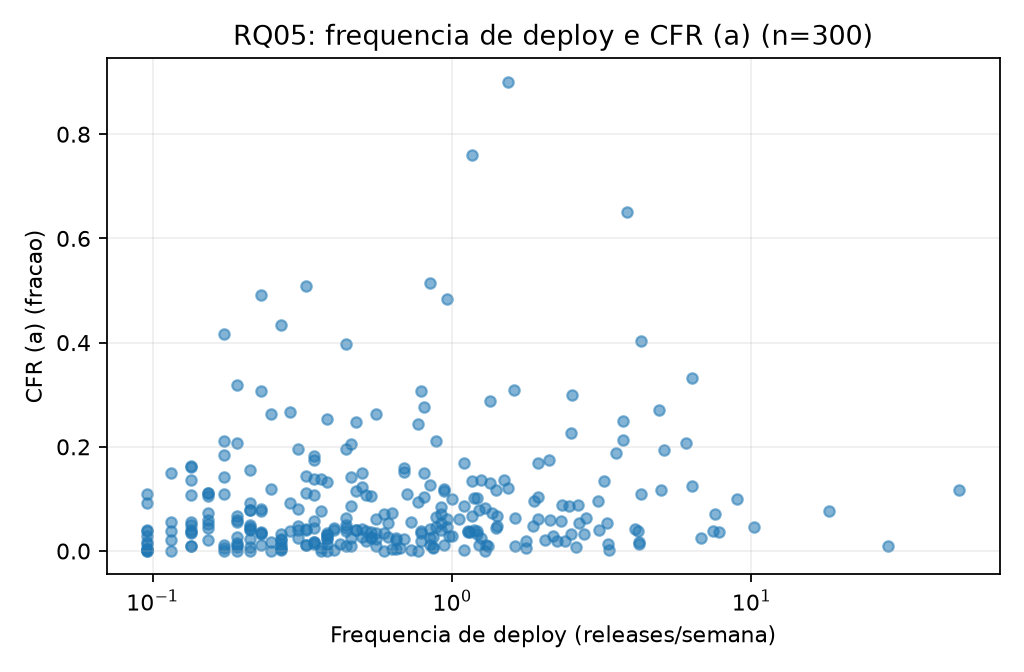
\includegraphics[width=.48\textwidth]{assets/rq05_frequencia_cfr_a.png}\hfill
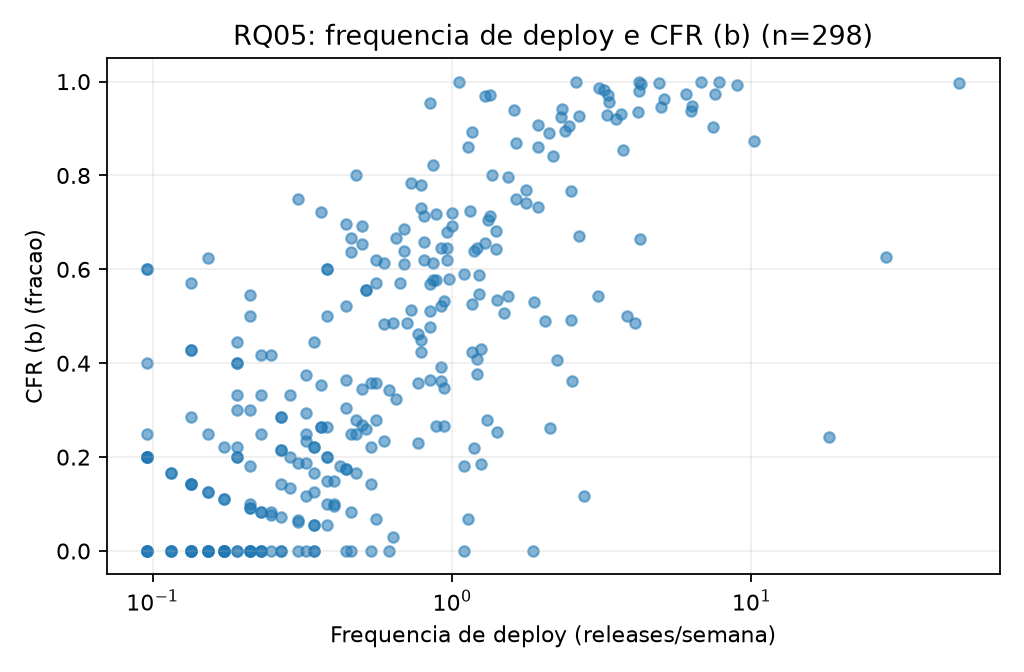
\includegraphics[width=.48\textwidth]{assets/rq05_frequencia_cfr_b.png}
\caption{Frequência de deploy (escala log) versus CFR (a), à esquerda, e CFR (b), à direita.}\label{fig:rq05}
\end{figure}

Na RQ06, após a correção de Holm, só o lead time (a) difere entre grupos: por quartil de contribuidores ($p_{Holm} < 10^{-10}$, $\varepsilon^2 = 0{,}19$) e por linguagem ($p_{Holm} = 0{,}0006$, $\varepsilon^2 = 0{,}09$). O quartil com mais contribuidores tem lead time (a) \textbf{maior} que Q1 (Cliff's $\delta = -0{,}65$, grande), Q2 ($-0{,}52$, grande) e Q3 ($-0{,}38$, médio). Go e o grupo ``outras'' têm lead time (a) maior que Python e TypeScript ($\delta$ entre 0,35 e 0,44, médio). Estrelas e tipo do projeto ($n = 60$) não mostraram diferença significativa em nenhuma métrica.

\subsection{RQ07: sensibilidade às definições}

\begin{table}[ht]
\centering
\caption{Mudança de categoria geral entre combinações de definições ($n = 300$).}\label{tab:rq07}
\small
\begin{tabular}{lrrr}
\toprule
Par & Mudaram & \% & Kappa ponderado \\
\midrule
C1 $\times$ C2 & 114 & 38,0 & 0,41 \\
C1 $\times$ C3 & 61 & 20,3 & 0,71 \\
C2 $\times$ C3 & 117 & 39,0 & 0,44 \\
\bottomrule
\end{tabular}
\end{table}

Entre C1 e C2, a nota de CFR muda para 73\% dos repositórios e a de lead time para 41\%; a de frequência, para 11\% (Tabela~\ref{tab:rq07}). As distribuições gerais passam de 14/130/132/24 (Low/Medium/High/Elite) em C1 para 20/188/89/3 em C2 e 9/108/160/23 em C3. As inferências por subgrupo também mudam: contribuidores estão associados à categoria geral em C1 ($p_{Holm} = 0{,}028$), mas não em C2 nem C3, e linguagem só em C3 ($p_{Holm} = 0{,}011$).

\subsection{RQ08 (bônus): \textit{rework rate}}

A proporção de releases corretivas, pela mesma heurística do CFR (b), tem mediana de 72\% por repositório (Q1 41\%, Q3 90\%); são 12.242 das 22.130 releases. Diferentemente do CFR (b), que conta a release que \textbf{precedeu} uma correção em até 7 dias, o \textit{rework rate} conta a própria correção, sem limite de tempo e incluindo as releases censuradas; as duas taxas respondem a perguntas diferentes.

\section{Discussão}

\textbf{H01 confirmada em parte.} A mediana é \textit{Medium} e só 8 repositórios são \textit{Elite}, como esperado; mas 65 (22\%) são \textit{Low}, com menos de uma release por mês, mais do que esperávamos para projetos tão ativos. Releases de projetos populares são semanais a mensais, não contínuas.

\textbf{H02: faixa confirmada, divergência refutada.} As medianas ficam entre 1 e 30 dias, mas a variante (b) não é menor que a (a): a mediana de (b) é até um pouco maior (11,1 contra 10,5 dias), e (a) supera (b) em apenas 177 dos 299 repositórios. Em cada release, (a) é sempre $\ge$ que os valores de (b), pois usa o commit mais antigo. No repositório, porém, (a) dá peso igual a cada release, enquanto (b) dá peso a cada commit: as releases longas, com muitos commits acumulados, dominam a mediana de (b). O efeito do commit ``esquecido'' existe por release, mas é compensado por essa diferença de pesos.

\textbf{H03 refutada nas duas variantes.} O CFR (a) é baixo (4,8\%) porque os runs considerados são de \texttt{push} no \textit{default branch}: as falhas acontecem antes, nos \textit{pull requests}, e o que chega ao branch principal já passou pelo CI. O CFR (a) mede, portanto, quebras do pipeline após o merge, e não falhas percebidas por usuários em produção. O CFR (b) é alto (36\%) porque projetos populares publicam correções logo após as releases. Ele está mais próximo de ``falha em produção'', mas é limitado pela heurística e pela ambiguidade do próprio conceito de release corretiva ($\kappa = 0{,}09$).

\textbf{H04 confirmada.} A recuperação mediana de 2,6 horas é \textit{High}; a maioria das quebras no branch principal é corrigida no mesmo dia.

\textbf{H05 refutada.} As duas correlações são positivas. Com o CFR (a) a associação é fraca, compatível com a afirmação do DORA de que velocidade não exige sacrificar estabilidade. Com o CFR (b) a associação forte é, em parte, mecânica: quem publica mais releases tem mais chances de que uma correção caia nos 7 dias seguintes a cada release. Correlação não implica causalidade.

\textbf{H06 refutada.} Mais contribuidores se associam a lead time \textbf{maior}, não menor; estrelas e tipo do projeto não fazem diferença detectável. Uma explicação plausível é que projetos grandes acumulam mais commits por release e mantêm \textit{branches} de release (155 repositórios têm releases cuja anterior por data não é ancestral), o que alonga o intervalo entre o commit e a publicação.

\textbf{H07 confirmada.} De 20\% a 39\% dos repositórios mudam de categoria, e o kappa ponderado vai de moderado (0,41) a substancial (0,71). O que mais move a classificação é a definição de falha: comparações que mantêm o CFR (a) concordam bem mais. Assim, as conclusões das RQ01 a RQ04 sobre velocidade são relativamente robustas, enquanto as que envolvem falha (RQ03 b, RQ05 b) e as inferências por subgrupo (RQ06) dependem da definição escolhida. A maior surpresa foi a validação manual: três pessoas lendo as mesmas notas e commits discordaram sobre o que é uma release corretiva quase tanto quanto o acaso.

\section{Ameaças à validade}\label{sec:ameacas}

\textbf{Validade de construto.} A principal ameaça reside na aderência dos \textit{proxies}: releases oficiais não correspondem diretamente a deploys em produção no caso de bibliotecas ou frameworks, e o CFR (a) reflete quebras de integração contínua após o merge na branch principal, não incidentes operacionais percebidos por usuários finais. A heurística de identificação de releases corretivas foi calibrada contra um consenso de três avaliadores caracterizado por alta prevalência de correções (79\%) e concordância interavaliador apenas leve ($\kappa = 0{,}09$); sob essa assimetria, até classificadores ingênuos alcançam F1 elevado, exigindo que o F1 obtido (0,82) seja interpretado em conjunto com a precisão (0,91) e com os F1s individuais (0,72 a 0,81). Além disso, a discrepância entre as taxas individuais de marcação (49\% a 85\%) comprova a ambiguidade inerente à definição manual de correção. Na medição de lead time, práticas de desenvolvimento baseadas em \textit{rebase} ou \textit{squash merge} distorcem o campo \texttt{commit.author.date}: identificamos 1.553 commits (em 4 milhões) cuja autoria antecede historicamente eventos passados mas cujo registro cronológico resultou em valor formalmente posterior à release (lead time nominalmente negativo, preservados sem descarte artificial para não enviesar a mediana).

\textbf{Validade interna.} A existência de ramificações complexas e \textit{release branches} resultou em comparações de histórico classificadas como \texttt{diverged} em 155 repositórios (3.270 releases, 15\% do total), nas quais a API do GitHub compara a partir do mais recente ancestral comum, modelo estatisticamente distinto de históricos estritamente lineares. Releases redundantes vinculadas ao mesmo commit da versão predecessora (3.538 ocorrências) foram excluídas do cálculo de lead time por representarem apenas retagging. Cinco comparações retornaram código HTTP 404 devido a tags posteriormente removidas por mantenedores remotos, e uma resposta apresentou paginação truncada da API. Fatores de confusão históricos decorrem da idade dos projetos: repositórios maduros acumulam concomitantemente maior volume de releases e base mais ampla de colaboradores. Por fim, para evitar distorções decorrentes de execuções paginadas concorrentes à publicação de novos artefatos, duplicatas geradas durante janelas de paginação foram identificadas e saneadas. A análise de sensibilidade evidenciou que a classificação DORA é altamente volátil à definição de falha (mudança de categoria em 38\% dos projetos entre C1 e C2), demonstrando que conclusões operacionais dependem estritamente da métrica de estabilidade adotada.

\textbf{Validade externa.} O estudo restringiu-se estritamente ao estrato de elite do ecossistema de código aberto hospedado no GitHub, composto pelos repositórios mais populares que utilizam GitHub Actions ($\ge 40.000$ estrelas). Consequentemente, as conclusões empíricas, taxas de falha pós-merge e tempos de ciclo não são generalizáveis a projetos de menor visibilidade, repositórios corporativos ou sistemas internos nos quais práticas de deploy contínuo em nuvem e telemetria de produção são monitoradas de ponta a ponta.

\textbf{Validade de conclusão.} Para mitigar o risco de conclusões espúrias decorrentes de 16 contrastes estatísticos simultâneos na RQ06, aplicou-se a correção estrita de Holm-Bonferroni sobre os p-valores de Kruskal-Wallis e Mann-Whitney. A tipologia do projeto baseou-se exclusivamente na amostra-ouro ($n = 60$), conferindo menor poder aos testes desse subgrupo. Ademais, o coeficiente kappa para verificação de ``entregas reais'' revelou-se matematicamente indeterminado em virtude da ausência de variabilidade nas respostas dos avaliadores. Finalmente, enfatiza-se que as associações de Spearman calculadas para a RQ05 denotam correlações empíricas e não constituem relação causal de causalidade.

\section{Replicação cruzada}\label{sec:replicacao}

\textbf{Infraestrutura e reprodutibilidade.} Para viabilizar a replicação cruzada cega preconizada na Seção~9 das diretrizes do projeto, desacoplou-se a camada de mineração da fase exploratória de busca: o pipeline foi estendido com os parâmetros \texttt{--repositorios} (alimentado por uma lista fixa de alvos) e \texttt{--saida} (isolando os artefatos de dados e persistência de cache). Adicionalmente, disponibilizou-se o módulo \texttt{comparar\_datasets.py}, encarregado de quantificar automaticamente a divergência relativa por métrica ($|replicado - original| / |original|$) e a concordância ordinal da categorização DORA sob tolerância de 10\%.

\textbf{Autorreplicação empírica.} Como prova de conceito e validação do protocolo antes da entrega final, o grupo realizou uma autorreplicação independente: executou-se o pipeline com cache rigorosamente limpo sobre uma subamostra determinística de 30 repositórios do dataset original (\texttt{random\_state = 42}). O processamento consumiu 8.593 requisições da API e concluiu-se em 1 hora e 20 minutos sem requerer nenhuma intervenção manual. A confrontação automatizada com o dataset de referência atestou 100\% de concordância na classificação DORA dos 30 repositórios e diferença relativa nula (0,000) em todas as seis métricas contínuas observadas na janela fixa (frequência, lead time variantes a/b, CFR variantes a/b e recuperação). Pequenas variações detectaram-se unicamente nas contagens acumuladas de estrelas e colaboradores totais, decorrentes de sua medição em tempo real na data de execução. O resultado confirma a robustez e a total reprodutibilidade do arcabouço metodológico sob janela temporal fechada.

\textbf{Status da replicação externa.} Conforme estipulado no planejamento da disciplina, a etapa de replicação externa previa a execução cruzada do código de outro grupo de alunos. Todavia, até a data-limite de submissão do trabalho, o repositório e o artefato do grupo externo parceiro não foram designados nem disponibilizados pela coordenação docente. Do mesmo modo, nenhuma issue de divergência técnica foi submetida por terceiros contra o nosso repositório. O ferramental de execução e análise de conformidade permanece plenamente operacional e versionado no projeto caso dados externos venham a ser fornecidos subsequentemente.

\section{Repositório e quadro do projeto}

Código-fonte, dados minerados e documentação técnica encontram-se publicamente acessíveis no repositório GitHub: \url{https://github.com/JoaoRajao/lab-medicao} (diretório \texttt{labs/lab03\_dora}). O acompanhamento evolutivo das tarefas e o quadro Kanban da equipe estão registrados no GitHub Projects: \url{https://github.com/users/JoaoRajao/projects/4}.

\bibliographystyle{sbc}
\begin{thebibliography}{99}
\bibitem{forsgren2018accelerate}
Forsgren, N., Humble, J., \& Kim, G. (2018). \textit{Accelerate: The Science of Lean Software and DevOps}. IT Revolution.

\bibitem{dora2024history}
DORA. (2024). \textit{A history of DORA's software delivery metrics}. Disponível em: \url{https://dora.dev/insights/dora-metrics-history/}.

\bibitem{landis1977}
Landis, J. R. \& Koch, G. G. (1977). The measurement of observer agreement for categorical data. \textit{Biometrics}, 33(1):159--174.

\bibitem{romano2006}
Romano, J. et al. (2006). Appropriate statistics for ordinal level data. \textit{Annual Meeting of the Florida Association of Institutional Research}.

\bibitem{wohlin2012}
Wohlin, C. et al. (2012). \textit{Experimentation in Software Engineering}. Springer.
\end{thebibliography}

\end{document}
